% siminos/spatiotemp/Examples/examReflectA.tex
% $Author: predrag $ $Date: 2021-08-10 11:56:19 -0400 (Tue, 10 Aug 2021) $

\renewcommand{\Refl}{\ensuremath{{\sigma}}} % conflict with ``symmetric''

%%%%%%%%%%%%%%%%%%%%%%%%%%%%%%%%%%%%%%%%%%%%%%%%%%%%%%%%%%%%%%%%%%
\example{A reflection--symmetric  $1d$ map.}{
\label{exam:ReflectA} %was {dscr:ReflectA}
% in examFiniteGr.tex, called by \Chapter{finiteGr}{}{Flips, slides and turns}
        \index{sawtooth map}\index{map!sawtooth}             \toCB
Consider a 1\dmn\ bimodal `sawtooth' map $\map$ shown in
\reffig{dscr:f_1d_symm_A}.
\beq
\ssp_{\zeit+1} =
% \flow{}{\ssp_{\zeit}} =
\left\{ \begin{array}{ll}
        f_L(\ssp_{\zeit}) =  \ExpaEig(\ssp_{\zeit}+1)-1  \,, \quad
                                    & \ssp_{\zeit} \in \pS_0=[-1,-\ell/2) \\
        f_C(\ssp_{\zeit}) =  \ExpaEig_C \ssp_{\zeit} \,, \quad
                                    & \ssp_{\zeit} \in \pS_0=[-\ell/2,\ell/2] \\
        f_R(\ssp_{\zeit}) =  \ExpaEig(\ssp_{\zeit}-1)+1 \,, \quad
                                    & \ssp_{\zeit} \in \pS_1 =(\ell/2,1]
        \,,
         \end{array}\right.
\ee{symmBimod}
with $\ell=2/|\ExpaEig_C|$, and $2/|\ExpaEig|+1/|\ExpaEig_C|=1$. The map is piecewise-linear on the \statesp\
$\pS = [-1,1]$, a compact 1-dim\-ens\-ion\-al line interval, split into
three regions $\pS = \pS_L \cup \pS_C \cup \pS_R$.
% (the labels stand for $L$(eft), $C$(enter), and $R$(ight)).
    %
%%%%%%%%%%%%%%%%%%%%%%%%%%%%%%%%%%%%%%%%%%%%%%%%%%%%%%%%%%%%%%%
%\SFIG{bimodTraj}{}{
\FIG{
(a)~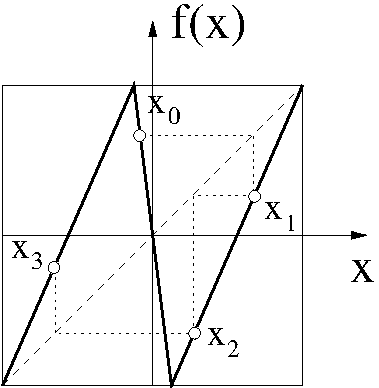
\includegraphics[width=0.35\textwidth]{bimodTraj-a}
(b)~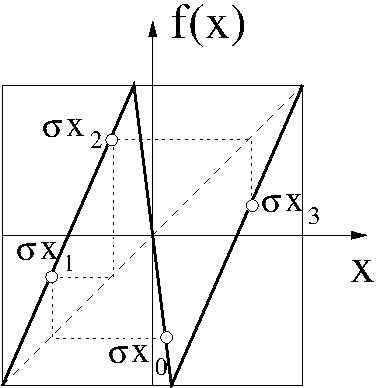
\includegraphics[width=0.35\textwidth]{bimodTraj-b}
}{}{
The bimodal Ulam sawtooth map with the $\Dn{1}$ symmetry $f(-\ssp)=-f(\ssp)$.
If the trajectory (a)
$\ssp_0 \to \ssp_1 \to \ssp_2 \to \cdots$ is a solution,
so is its reflection (b)
$\Refl\ssp_0 \to \Refl\ssp_1 \to \Refl\ssp_2 \to \cdots$.
~~(work through \refexam{exam:ReflectA};
continued in \reffig{dscr:f_1d_symm_a}).
}{dscr:f_1d_symm_A}
%%%%%%%%%%%%%%%%%%%%%%%%%%%%%%%%%%%%%%%%%%%%%%%%%%%%%%%%%%%%%%%
    %
    % finiteGrD1.mp4             length  13:11
    % Title:  Example: a 1-dimensional system with a symmetry
    % [2015-01-28 Predrag} clipped
    % re-recording and replacement for discrete1D1.mp4
    % 4:29 write "false claim - this is not a fixed point!"
\toVideo{youtube.com/embed/sI39jMdjxVM} % uploaded 2015-01-04
    %
The map is reflection-symmetric, $\map(-\ssp) = - \map(\ssp)$.

Denote the reflection operation by $\Refl\ssp = - \ssp$.
The 2-element
group $\Group=\{e,\Refl\}$ goes by many names, such as $Z_2$ or $\Cn{2}$.
Here we shall refer to it as $\Dn{1}$, dihedral group generated by a single
reflection. The $\Group$-equivariance of the map implies that if
$\{\ssp_n\}$ is a trajectory, than also $\{\Refl\ssp_n\}$ is a
symmetry-equivalent trajectory because
$
\Refl\ssp_{n+1} = \Refl f(\ssp_n) = f(\Refl \ssp_n)
\,.
$

In the temporal lattice formulation, there is a triplet of fields
\(
\field_\zeit=(\field^{L}_{\zeit},\field^{C}_{\zeit},\field^{R}_{\zeit})
\)
at each lattice site $\zeit$.
Just like the temporal Bernoulli \refeq{diffEqs:1stepDiffEq},
temporal {\lattstate}s satisfy a linear first-order difference equation
\beq
\field_{\zeit} - \map\circ\field_{\zeit-1} = 0
\,,
\ee{sawtooth:1stepDiffEq}
but now for a triplet of fields satisfying the local condition
\refeq{symmBimod} at each lattice site. As the local slope can be either
$\ExpaEig$ or $\ExpaEig_C$, the $[3\cl{}\!\times\!3\cl{}]$ {\jacobianOrb}
$\jMorb$ takes a block-diagonal form, and depends on the symbol \brick\
of a particular {\lattstate}.
\bigskip

{\color{red}Challenge}: write down the \HillDet\ for a given symbol \brick,
not only using Hill's formula, but also directly, without time evolution.

~~(continued in \refexam{exam:Reflecti})
    \PC{2021-06-12}
       {write up exercise {exer:ReflectA}: write down the formula for
        the map of \reffig{dscr:f_1d_symm_A}, verify its $\Dn{1}$-equivariance.}
                                        \jumpBack{exam:ReflectA}
} %end \example{A reflection symmetric $1d$ map:
%%%%%%%%%%%%%%%%%%%%%%%%%%%%%%%%%%%%%%%%%%%%%%%%%%%%%%%%%%%%%%%%%%

\renewcommand{\Refl}{\ensuremath{{s}}} % Dihedral wiki convention
